\subsection*{Resultater}
Fra app'ens hovedmenu kan brugeren tilgå sine resultater. På denne måde er det muligt for brugeren at få et overblik over udviklingen samt udførte træninger.
Aktivitetsdiagrammet over resultater fremgår af \autoref{fig:resultater}.

\begin{figure} [H]
\centering
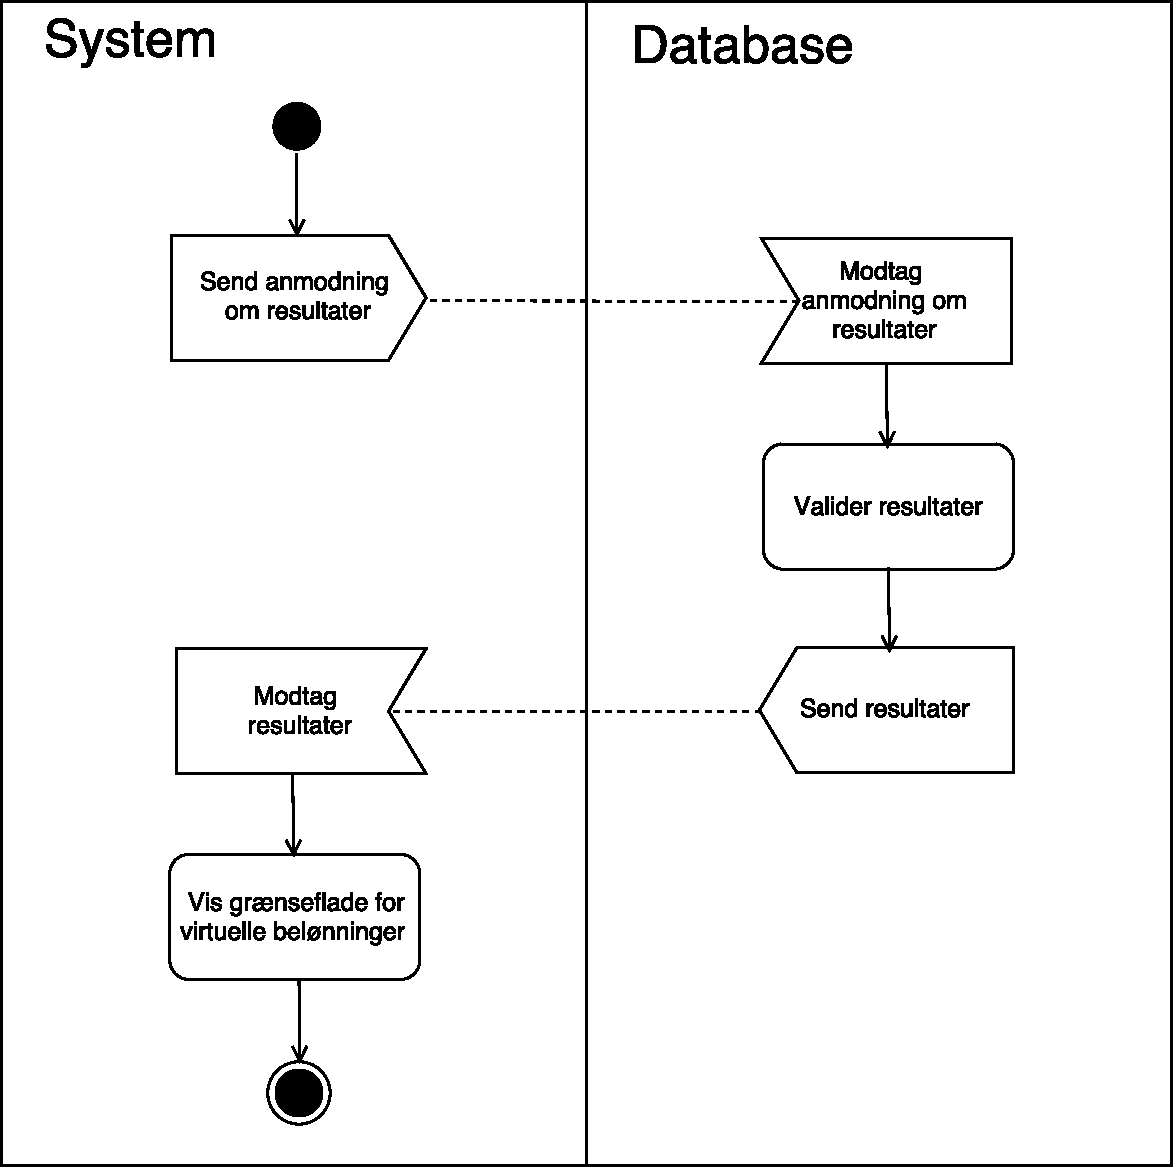
\includegraphics[width=0.9\textwidth]{figures/aktivitetsdiagram/Resultater}
\caption{Aktivitetsdiagram over resultater.}
\label{fig:resultater}
\end{figure}

\noindent
I resultater er det muligt for brugere at følge sin udvikling, hvor ofte de træner, samt hvilke belønneringer de har opnået. 
Brugere kan i kalenderen få overblik over, hvilke dage, der er udført træning samt tilgå tidligere træningsresultater. I belønninger kan brugere se, hvilke virtuelle belønninger de har opnået i forbindelse med træning. Belønningerne varierer afhængig af træningsform. Inden for hver træningsform, jf. \autoref{sec:traening}, kan der opnås beløninger inden for forskellige kategorier. Et eksempel på fordeling af belønninger i forskellige kategorier fremgår af \autoref{tab:beloenninger}.

\begin{table} [H]
\centering
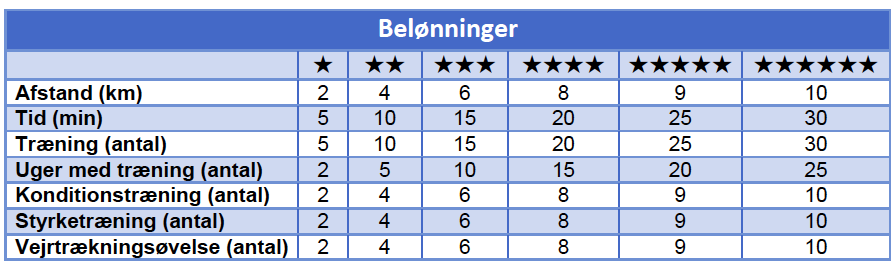
\includegraphics[width=1\textwidth]{figures/aktivitetsdiagram/beloeninnger}
\caption{Eksempel på belønninger opnået ved træning inden for forskellige kategorier.}
\label{tab:beloenninger}
\end{table}

\noindent
Ud fra \autoref{tab:beloenninger} fremgår et eksempel på fordeling af virtuelle belønninger, der er opdelt efter afstand, tid og antallet af gennemførte træninger. 